The system is based upon the fact that no single node knows where can a file be 
found. With this in mind, a distributed searching procedure or algorithm is 
needed every time a file needs to be found somewhere in the network of peers.

Basic idea: When a node A asks a node B if it can provide file F, and then B 
replies with "yes", node A can't know if B has F or it just simply forwards the 
reply of another node C, which has F, but it's unknown to A. In fact, the "yes" 
in this case really means that B is a proxy located in the path between the 
requester (A) and the provider (C), and thus can facilitate communication 
between the two parties which are unknown to each other. This procedure can be 
applied recursively, which means that such proxy paths of arbitrary length (or 
depth) can be obtained. To avoid cycles, each request will contain a unique 
randomly generated identifier. If a node encounters a request identifier for 
the second time, it won't forward it again. Figure \ref{fig:fig4} illustrates a 
search with a maximum depth of two, initiated by node N1. The nodes N7 and N8 
have the requested file.

\begin{figure}
    \centering
    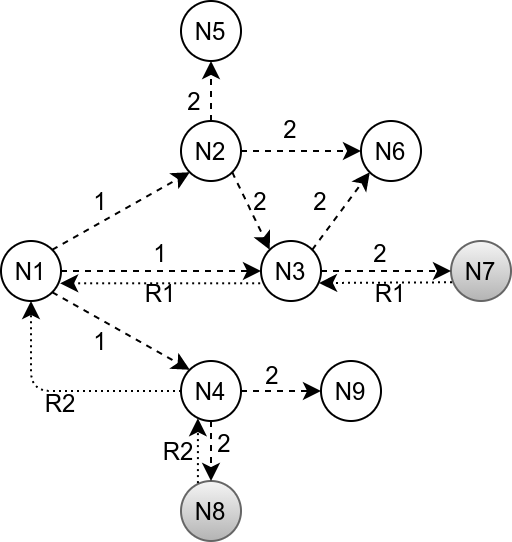
\includegraphics[width=0.4\textwidth]{figures/fig4}
    \caption{Run of the file searching algorithm with a maximum depth of two}
    \label{fig:fig4}
\end{figure}

\subsection{Request Table}

In order for a node to be part of a search request path, it needs to remember 
where the request came from. When a reply which contains the same request 
identifier arrives, the node will know where to direct it based on the 
association between the request identifier and the local request origin 
address. The list of these associations is called \textit{Request Table}. When 
a reply has been satisfied locally, the entry should not yet be removed, 
because another reply for the same request might be issued by another node.

The key reason why multiple responses to the same request are collected is that 
if, for some reason, the file provider disconnects, the requesting node may 
have backups for the transfer. Besides that, a future version of the protocol 
might support retrieving a file from multiple providers at the same time 
(similar to BitTorrent). An entry from the Request Table might have an 
expiration time, after which it can be deleted.

\subsection{Reply Table}

The requesting node will have to confirm the transfer with one of the file 
providers by sending a confirmation through the same path as the request. In 
order to allow such a scheme for confirmations, replies coming back through a 
path will have to be saved along with each hop. Let each reply have a unique 
identifier. When a node is on a reply path, it remembers the reply identifier 
and its origin in a \textit{Reply Table} (similar to the Request Table). A 
transfer confirmation will then have to contain the reply identifier 
corresponding with the route to the file provider. After a reply identifier is 
used within a confirmation message to forward it, the corresponding entry in 
the Reply Table can be removed. The other replies associated with the request 
from which they originated will still have to be kept in the Reply Table for 
the same reasons stated in the previous subsection.

\subsection{Encryption}

The reply contains sensitive information, like the \textit{Transfer Key} and 
\textit{Rendezvous Addresses}, which are used for the actual file transfer and 
will be discussed in the following section. To avoid snooping by potential 
adversaries located in the search path, the sensitive information has to be 
encrypted using a public key scheme. A public key is appended to the request 
message, which is used by the file provider to encrypt the sensitive 
information from the reply. The request sender can obtain that information by 
decrypting it using its private key (figure \ref{fig:fig5}).

\begin{figure}
    \centering
    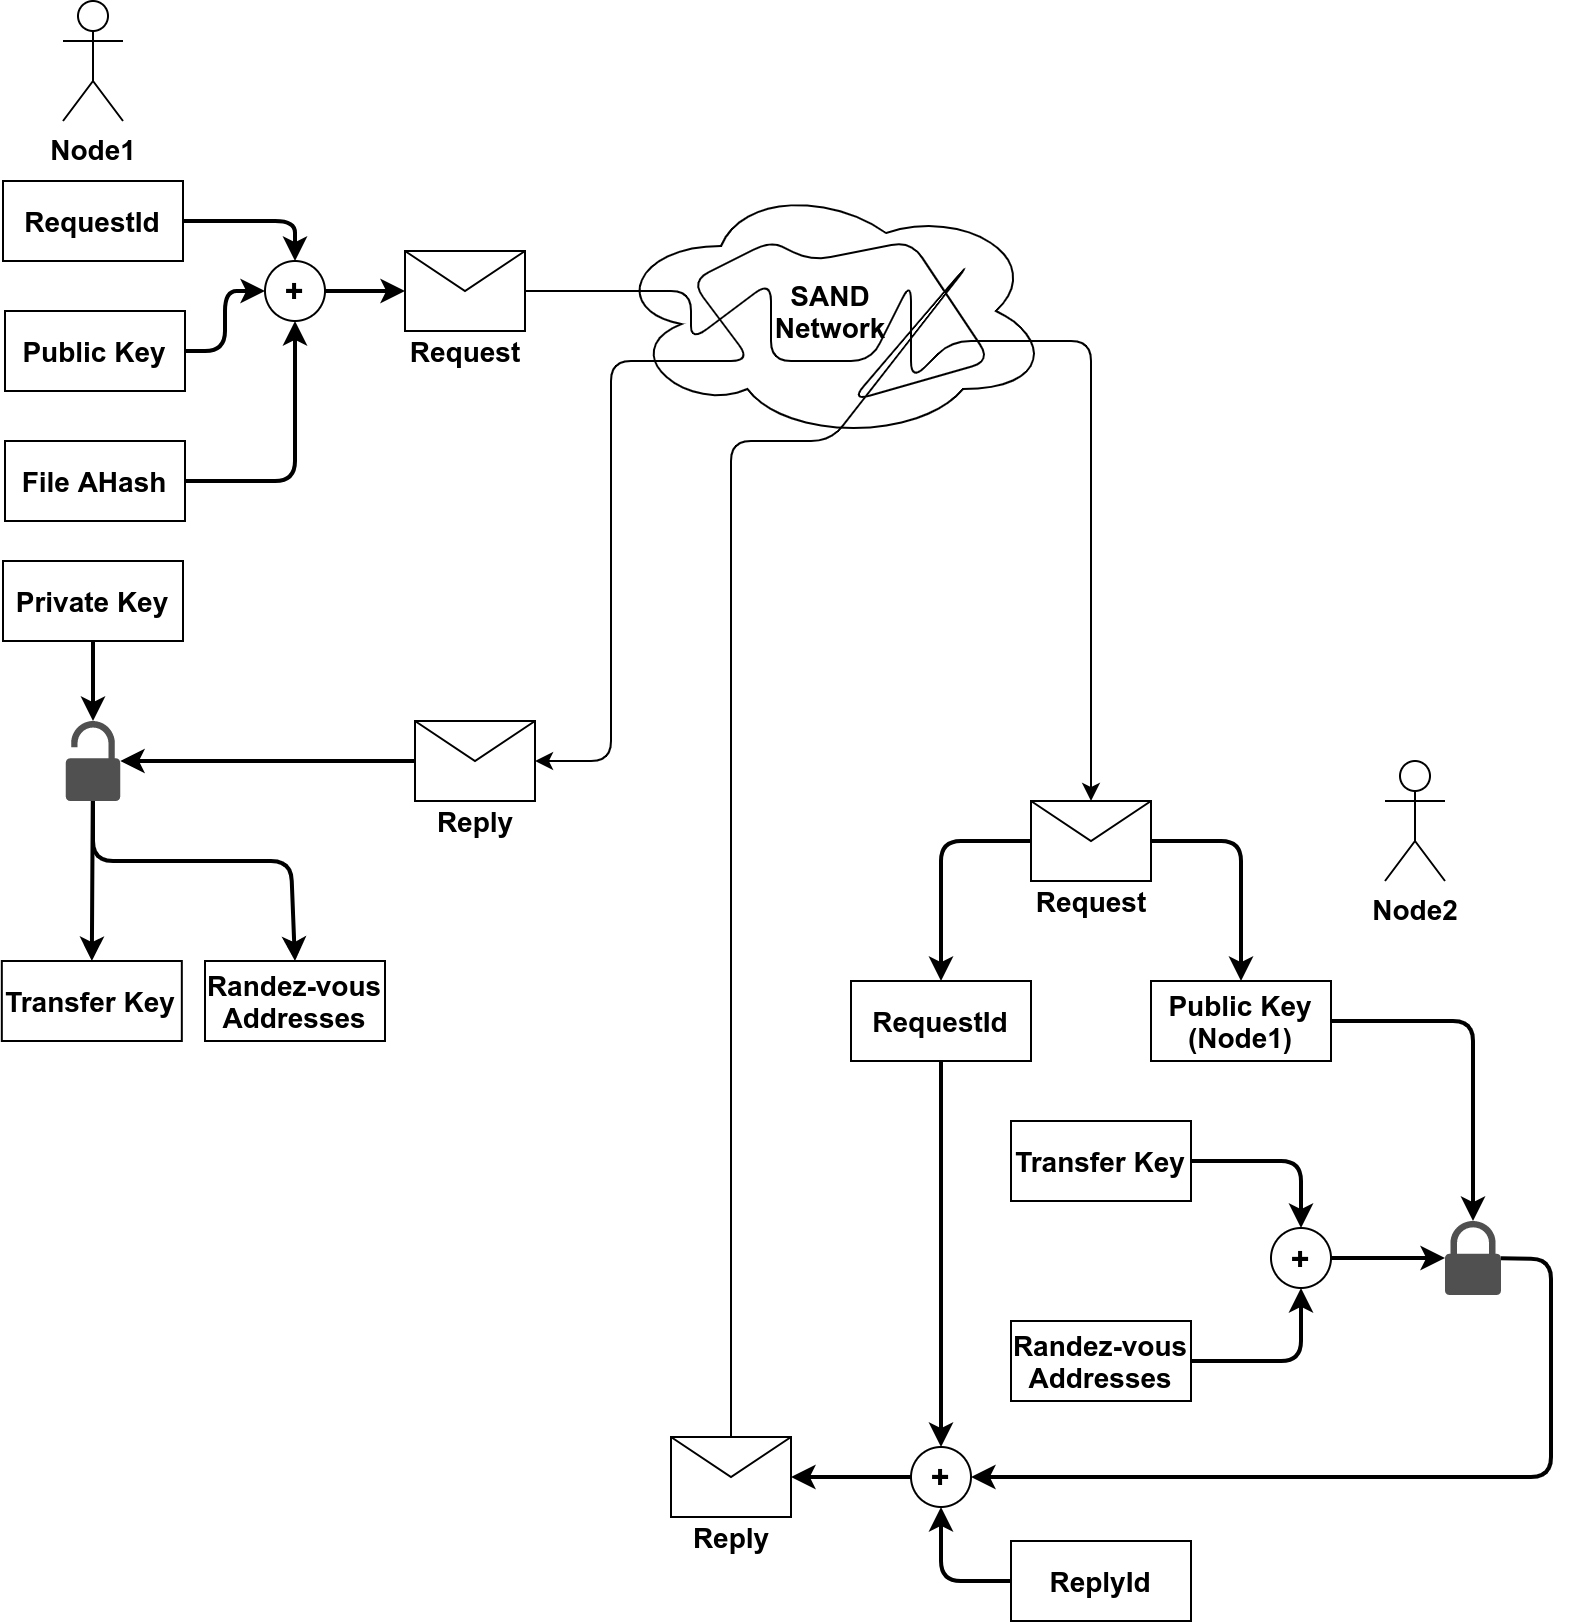
\includegraphics[width=\textwidth]{figures/fig5}
    \caption{Search request and reply}
    \label{fig:fig5}
\end{figure}

The key pair should be regenerated for every search query to greatly reduce the 
risk of identifying the search initiator.

\subsection{Path Caching}

Popular files could be requested multiple times and thus, to improve 
performance and to decrease network congestion, a route caching mechanism is 
proposed. When a reply passes through a node, indicating the requested file was 
found on the current path, this information is saved in a local \textit{Path 
Cache}. An entry in this cache contains the file AHash and the addresses which 
represent the continuation of the paths to the file provider. When a request 
for the same file is received the cache is consulted then, the request is 
forwarded only to the nodes indicated in the cache entry.

There are two primary problems with this approach:
\begin{itemize}
    \item A node in the cached path may go offline and thus invalidate the 
cache. The solution, in this case, would be to send a special message back 
along the path which indicates the cache is invalidated.
    \item New nodes may appear in the network which could create new potential 
paths. The simplest solution here is to implement a cache expiration mechanism.
\end{itemize}

\begin{figure}
    \centering
    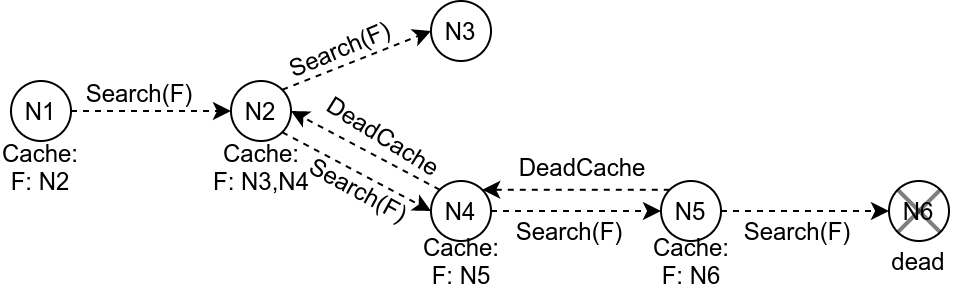
\includegraphics[width=0.7\textwidth]{figures/fig6}
    \caption{Dead node in a cached path}
    \label{fig:fig6}
\end{figure}

Figure \ref{fig:fig6} illustrates a scenario in which a node from a cached path 
goes offline. \textit{DeadCache} messages are sent back along the path. N2 does 
not forward the DeadCache message because the cached path going through N3 is 
still valid, so N2 remains part of a cached path. Nodes N4 and N5 will remove 
their entries for file F, while N2 will merely remove node N4 from the entry.
